% =====================================================================
% Tercera parte – 1 a 5. Introducción y métricas internas
% =====================================================================
\section{Introducción}

Medir el software es asignar valores numéricos a atributos del producto para evaluarlo, compararlo y mejorarlo con criterios repetibles \parencite{fenton2014}. Las métricas \textbf{internas} (tamaño, complejidad, acoplamiento y cohesión) se calculan sobre el código sin ejecutarlo y anticipan la mantenibilidad. Las métricas \textbf{externas} se observan con el producto en ejecución y siguen el modelo de calidad de ISO/IEC 25010 \parencite{iso25010}, con las medidas de ISO/IEC 25023 \parencite{iso25023}.

Cada métrica se calculó dos veces: sobre el commit \codigo{0efe28b} (\textbf{antes}, el código de la entrega anterior) y sobre la rama \codigo{fix/defectos} (\textbf{después} de la refactorización y las correcciones). Así se ve el efecto de las mejoras.

\section{Objetivos}

\begin{itemize}
  \item Cuantificar el tamaño de ShiftCash por lenguaje y comparar tres herramientas de conteo.
  \item Calcular la suite de Chidamber y Kemerer (WMC, DIT, NOC, CBO, RFC y LCOM) y la complejidad ciclomática, compararlas con valores de referencia publicados y señalar las clases y módulos problemáticos.
  \item Medir cada requisito no funcional (Tabla \ref{tab:rnf}) con su métrica externa y su valor objetivo.
  \item Mostrar el antes y el después de las mejoras y proponer las que faltan.
\end{itemize}

\section{Alcance}

El tamaño se mide sobre todo el código del producto (backend, frontend, estilos y configuración), sin \codigo{node_modules}, \codigo{package-lock.json}, la carpeta \codigo{docs/} ni los recursos binarios; el código de pruebas se reporta aparte. Las métricas orientadas a clases se aplican al backend en Python, y la complejidad aproximada, también a los componentes JSX. Las métricas externas se aplican a la aplicación desplegada cuando es posible y, si no, a la ejecución local de la Segunda parte.

\section{Tipos de métricas y herramientas}

\begin{table}[H]
\caption{Modelos y herramientas de medición}
\label{tab:herramientas-metricas}
\footnotesize
\begin{tabularx}{\linewidth}{L{2.6cm} L{4.6cm} Y}
\toprule
Tipo & Modelo o métrica & Herramienta \\
\midrule
Tamaño & LOC físicas, en blanco, de comentario y de código & \codigo{wc -l}; \codigo{metricas.py tamano} (Apéndice \ref{ap:metricas}); pygount 3 \parencite{pygount2025}; SonarQube \parencite{sonarqube2025} \\
Complejidad & Complejidad ciclomática de McCabe \parencite{mccabe1976} & \codigo{metricas.py complejidad} (AST de Python) y \codigo{metricas.py frontend} (puntos de decisión en JSX) \\
Orientadas a clases & WMC, DIT, NOC, CBO, RFC y LCOM \parencite{chidamber1994}; LCOM4 \parencite{hitz1995} & \codigo{metricas.py ck} \\
Calidad externa & ISO/IEC 25010 y 25023 & pytest, Cypress, Selenium, JMeter, ZAP, Lighthouse 12.8.2 \parencite{lighthouse2025}, LambdaTest \\
\bottomrule
\end{tabularx}
\tablenote{Fuente: elaboración propia.}
\end{table}

\section{Métricas internas}

\subsection{Tamaño del código}

\begin{table}[H]
\caption{Tamaño del código del producto por lenguaje (\codigo{metricas.py tamano})}
\label{tab:tamano}
\footnotesize
\begin{tabularx}{\linewidth}{L{2.6cm} *{5}{>{\raggedleft\arraybackslash}X} *{2}{>{\raggedleft\arraybackslash}X}}
\toprule
 & \multicolumn{5}{c}{Después (rama \codigo{fix/defectos})} & \multicolumn{2}{c}{Antes (\codigo{0efe28b})} \\
\cmidrule(lr){2-6}\cmidrule(lr){7-8}
Lenguaje & Archivos & Físicas & En blanco & Coment. & Código & Archivos & Código \\
\midrule
CSS & 15 & 5\,785 & 825 & 217 & 4\,743 & 15 & 4\,738 \\
JSX & 28 & 4\,864 & 504 & 93 & 4\,267 & 28 & 4\,243 \\
Python & 18 & 1\,478 & 268 & 57 & 1\,153 & 14 & 1\,286 \\
JavaScript & 25 & 923 & 133 & 85 & 705 & 25 & 699 \\
JSON & 2 & 50 & 0 & 0 & 50 & 2 & 39 \\
YAML & 2 & 59 & 5 & 5 & 49 & 1 & 22 \\
HTML & 1 & 18 & 2 & 0 & 16 & 1 & 16 \\
\midrule
\textbf{Total} & \textbf{91} & \textbf{13\,177} & \textbf{1\,737} & \textbf{457} & \textbf{10\,983} & \textbf{86} & \textbf{11\,043} \\
Lógica (Python, JS y JSX) & 71 & 7\,265 & 905 & 235 & 6\,125 & 67 & 6\,228 \\
\midrule
Código de pruebas & 8 & 1\,044 & 220 & 59 & 765 & 0 & 0 \\
\bottomrule
\end{tabularx}
\tablenote{El backend tiene más archivos pero menos líneas: se separó la capa \codigo{services/} y se eliminaron la lógica duplicada y el código muerto. Fuente: elaboración propia.}
\end{table}

\begin{table}[H]
\caption{Comparación del tamaño según la herramienta}
\label{tab:tamano-herramientas}
\footnotesize
\begin{tabularx}{\linewidth}{L{3.6cm} L{2cm} L{2cm} Y}
\toprule
Herramienta y medida & Antes & Después & Qué cuenta \\
\midrule
\codigo{wc -l} (líneas físicas) & 13\,201 & 13\,119 & Saltos de línea; no cuenta la última línea de los archivos que no terminan en salto. \\
\codigo{metricas.py} (físicas) & 13\,263 & 13\,177 & Todas las líneas, incluidos los blancos y comentarios. \\
\codigo{metricas.py} (código) & 11\,043 & 10\,983 & Excluye blancos y comentarios de línea y de bloque. \\
pygount (código) & 9\,569 & 9\,532 & Reconoce el lenguaje con Pygments y clasifica cada línea con reglas propias; cuenta aparte las líneas vacías o de solo signos, por eso da menos. \\
SonarQube (Lines of Code) & 11\,000 aprox. (13\,000 líneas totales) & \resSonarLoc & Líneas con código, sin blancos ni comentarios. \\
\bottomrule
\end{tabularx}
\tablenote{En la entrega anterior el script reportaba 10\,972 líneas de código antes; la diferencia con 11\,043 viene de una detección más precisa de los comentarios de bloque en la versión actual del script. Fuente: elaboración propia.}
\end{table}

\begin{figure}[H]
\centering
\caption{Medición del tamaño con las tres herramientas (después)}
\label{fig:tamano-herramientas}
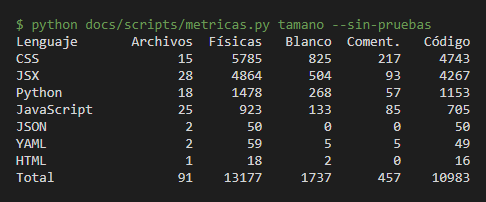
\includegraphics[width=0.48\linewidth]{../evidencias/metricas/script_tamano.png}\hfill
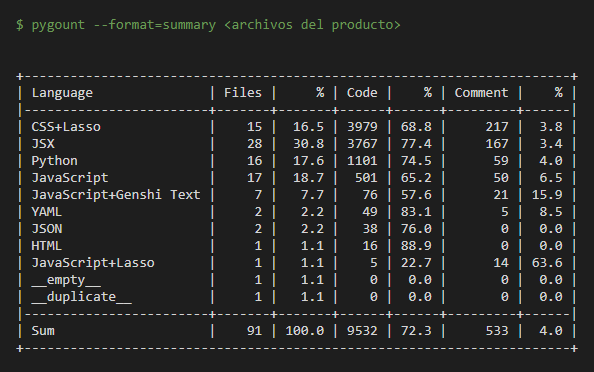
\includegraphics[width=0.48\linewidth]{../evidencias/metricas/pygount_tamano.png}\\[2mm]
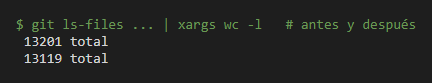
\includegraphics[width=0.48\linewidth]{../evidencias/metricas/wc_tamano.png}
\figurenote{Arriba: \codigo{metricas.py tamano} y pygount; abajo: \codigo{wc -l} (antes y después). Fuente: elaboración propia.}
\end{figure}

\begin{figure}[H]
\centering
\caption{Panel de SonarQube Community 26.7 (antes)}
\label{fig:sonar-tamano}
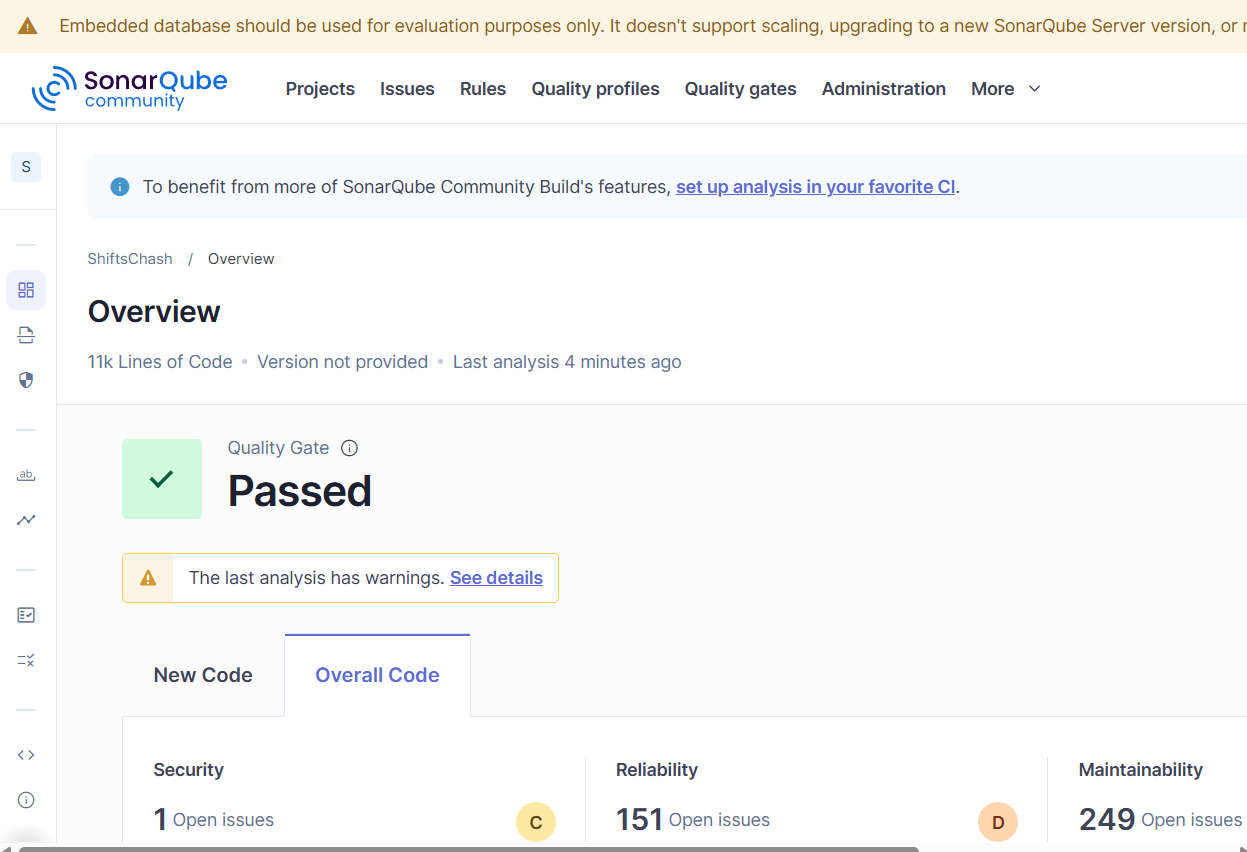
\includegraphics[width=0.8\linewidth]{previo/sonarqube_antes.png}
\figurenote{Fuente: elaboración propia.}
\end{figure}

\paragraph{Análisis.} Las tres herramientas coinciden en el orden de magnitud (entre 9\,500 y 11\,000 líneas de código) y difieren por lo que cada una considera código. El CSS es el 43\,\% del código, lo que refleja el peso de la presentación (tema claro y oscuro, diseño responsivo). La densidad de comentarios del Python bajó de 5,6\,\% a 3,9\,\% porque se borró el código comentado (el login antiguo), no porque se perdieran comentarios útiles; las clases y servicios nuevos tienen docstring.

\subsection{Complejidad ciclomática}

\begin{table}[H]
\caption{Complejidad ciclomática del backend}
\label{tab:complejidad}
\footnotesize
\begin{tabularx}{\linewidth}{L{5.2cm} Y Y}
\toprule
Medida & Antes & Después \\
\midrule
Funciones medidas & 58 & 92 \\
Funciones con $V(G) \leq 10$ \parencite{mccabe1976} & 55 (94,8\,\%) & 92 (100\,\%) \\
Funciones con $V(G) > 10$ & \codigo{update_saving_goal} (14), \codigo{get_date_range} (13), \codigo{update_budget} (13) & Ninguna \\
$V(G)$ máxima & 14 & 8 (\codigo{_toca_hoy}, \codigo{google_auth}) \\
$V(G)$ media & 3,4 & 2,2 \\
\bottomrule
\end{tabularx}
\tablenote{Según el catálogo de \textcite{filo2015}, una función es común con $V(G) \leq 2$, casual hasta 4 y poco común por encima de 4. Fuente: elaboración propia con \codigo{metricas.py complejidad}.}
\end{table}

\begin{table}[H]
\caption{Componentes del frontend con más puntos de decisión (después)}
\label{tab:frontend}
\footnotesize
\begin{tabularx}{\linewidth}{L{4.6cm} Y Y Y}
\toprule
Componente & Líneas & Funciones & Puntos de decisión \\
\midrule
PresupuestoModal.jsx & 466 & 33 & 83 \\
VistaResumen.jsx & 519 & 63 & 80 \\
VistaHistorial.jsx & 311 & 39 & 58 \\
VistaMetas.jsx & 367 & 33 & 46 \\
VistaConfiguracion.jsx & 385 & 24 & 45 \\
VistaPresupuestos.jsx & 409 & 40 & 43 \\
\bottomrule
\end{tabularx}
\tablenote{Puntos de decisión: \codigo{if}, \codigo{for}, \codigo{while}, \codigo{case}, \codigo{catch}, operador ternario, \codigo{\&\&} y \codigo{||}. Los valores son casi iguales a los de antes: la refactorización se concentró en el backend. Fuente: elaboración propia con \codigo{metricas.py frontend}.}
\end{table}

\subsection{Métricas orientadas a clases (suite CK)}

\paragraph{Definiciones aplicadas a Python.} Medimos las clases del backend (entidades SQLAlchemy y esquemas Pydantic) y, como la lógica de negocio está en funciones, también cada \textbf{módulo tratado como una clase}: sus funciones son los métodos y sus nombres globales, los atributos.
\begin{itemize}
  \item \textbf{WMC}: suma de las complejidades ciclomáticas de los métodos.
  \item \textbf{DIT}: profundidad de herencia hasta la clase raíz del marco (\codigo{Base} o \codigo{BaseModel} cuentan como nivel 1).
  \item \textbf{NOC}: número de subclases directas en el proyecto.
  \item \textbf{CBO}: número de otras clases o módulos del proyecto con los que se acopla (referencias o importaciones internas).
  \item \textbf{RFC}: métodos propios más funciones distintas que invocan.
  \item \textbf{LCOM}: pares de métodos sin atributos comunes menos pares con atributos comunes, mínimo 0 \parencite{chidamber1994}.
  \item \textbf{LCOM4}: componentes conexas del grafo de métodos, donde dos métodos se unen si comparten un atributo o uno usa al otro \parencite{hitz1995}. Vale 1 si la unidad es cohesiva.
\end{itemize}

\begin{table}[H]
\caption{Valores de referencia usados}
\label{tab:referencias-ck}
\footnotesize
\begin{tabularx}{\linewidth}{L{1.6cm} L{2.4cm} L{2.6cm} L{2.4cm} Y}
\toprule
Métrica & Común (bueno) & Casual (regular) & Poco común (malo) & Fuente \\
\midrule
WMC & $\leq 11$ & 12–34 & $> 34$ & \textcite{filo2015} \\
DIT & $\leq 2$ & 3–4 & $> 4$ & \textcite{filo2015} \\
NOC & $\leq 1$ & 2–3 & $> 3$ & \textcite{filo2015} (NSC) \\
CBO & $\leq 6$ & 7–16 & $> 16$ & \textcite{filo2015} (acoplamiento eferente) \\
NOM & $\leq 6$ & 7–14 & $> 14$ & \textcite{filo2015} \\
RFC & \multicolumn{3}{l}{Sin umbral numérico: «bajo», comparar con el resto} & \textcite{rosenberg1998} \\
LCOM4 & 1 & \multicolumn{2}{l}{$> 1$: responsabilidades separables} & \textcite{hitz1995} \\
$V(G)$ por función & $\leq 10$ & \multicolumn{2}{l}{$> 10$: dividir la función} & \textcite{mccabe1976} \\
\bottomrule
\end{tabularx}
\tablenote{Los umbrales de \textcite{filo2015} se derivaron de 111 sistemas Java; los usamos como referencia de lo habitual, no como reglas absolutas. Fuente: elaboración propia.}
\end{table}

\begin{table}[H]
\caption{Suite CK de las clases del backend (después)}
\label{tab:ck-clases}
\footnotesize
\begin{tabularx}{\linewidth}{L{3.2cm} L{2.2cm} *{7}{>{\centering\arraybackslash}X}}
\toprule
Clase & Tipo & NOM & WMC & DIT & NOC & CBO & RFC & LCOM4 \\
\midrule
User & Entidad & 0 & 0 & 1 & 0 & 4 & 0 & — \\
Category, Budget, Transaction & Entidad & 0 & 0 & 1 & 0 & 2 & 0 & — \\
SavingGoal & Entidad & 0 & 0 & 1 & 0 & 1 & 0 & — \\
SavingGoalCreate & Esquema & 4 & 10 & 1 & 0 & 0 & 10 & 3 \\
BudgetBase & Esquema & 4 & 5 & 1 & 2 & 0 & 9 & 4 \\
BudgetUpdate & Esquema & 4 & 6 & 1 & 0 & 0 & 9 & 4 \\
BudgetCreate & Esquema & 1 & 5 & 2 & 0 & 0 & 3 & 1 \\
TransactionCreate & Esquema & 3 & 6 & 1 & 0 & 0 & 7 & 3 \\
CategoryCreate, SavingGoalUpdate & Esquema & 2 & 4–5 & 1 & 0 & 0 & 5–6 & 2 \\
Otros 13 esquemas & Esquema & 0–1 & 0–2 & 1–2 & 0 & 0–1 & 0–4 & 0–1 \\
\midrule
Máximo (después / antes) & & 4 / 3 & 10 / 7 & 2 / 2 & 2 / 2 & 4 / 4 & 10 / 7 & 4 / 3 \\
\bottomrule
\end{tabularx}
\tablenote{Las entidades no tienen métodos, por lo que LCOM no aplica. El reporte completo, con LCOM, está en la Figura \ref{fig:ck}. Fuente: elaboración propia con \codigo{metricas.py ck}.}
\end{table}

\begin{table}[H]
\caption{Suite CK de los módulos del backend tratados como clases}
\label{tab:ck-modulos}
\footnotesize
\begin{tabularx}{\linewidth}{L{4.4cm} *{5}{>{\centering\arraybackslash}X} L{3.2cm}}
\toprule
Módulo & NOM & WMC & CBO & RFC & LCOM4 & Antes (NOM / WMC / RFC) \\
\midrule
routes/savings.py & 6 & 7 & 5 & 20 & 1 & 10 / \textbf{50} / 54 \\
routes/budgets.py & 4 & 5 & 5 & 17 & 1 & 6 / \textbf{37} / 35 \\
routes/transactions.py & 6 & 12 & 5 & 28 & 1 & 5 / 13 / 26 \\
routes/profile.py & 7 & 16 & 4 & 32 & 1 & Igual \\
routes/users.py & 3 & 14 & 4 & 23 & 1 & 3 / 16 / 23 \\
routes/categories.py & 4 & 7 & 5 & 19 & 1 & 4 / 6 / 19 \\
services/saving\_service.py & 14 & \textbf{39} & 2 & 63 & 3 & No existía \\
services/budget\_service.py & 12 & 25 & 3 & 40 & 4 & No existía \\
services/category\_service.py & 2 & 3 & 1 & 8 & 1 & No existía \\
auth.py & 4 & 7 & 2 & 20 & 3 & 4 / 8 / 21 \\
scheduler.py & 2 & 12 & 3 & 15 & 1 & Igual \\
\bottomrule
\end{tabularx}
\tablenote{En negrita, los valores poco comunes según \textcite{filo2015} (WMC $> 34$). Fuente: elaboración propia con \codigo{metricas.py ck}.}
\end{table}

\begin{figure}[H]
\centering
\caption{Reporte de la suite CK (después)}
\label{fig:ck}
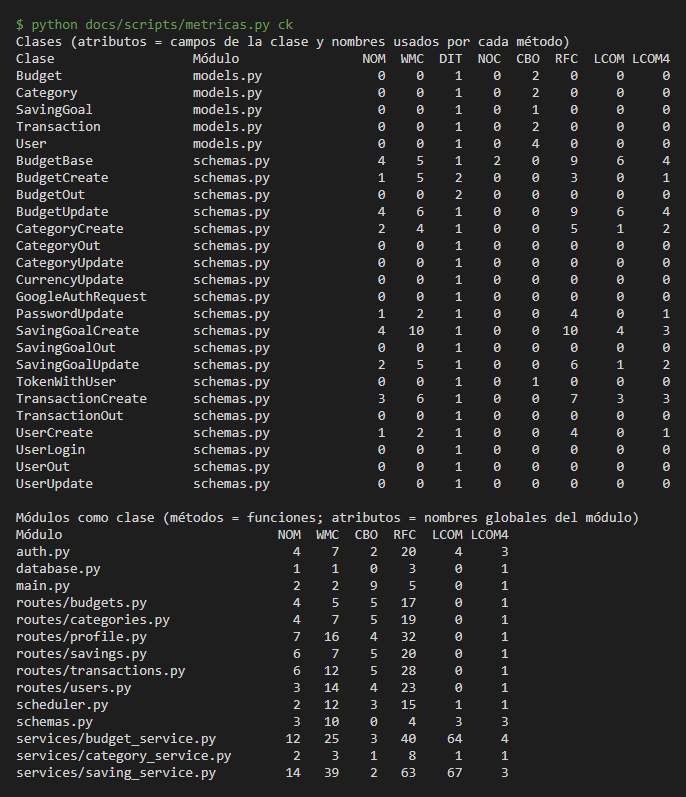
\includegraphics[width=0.75\linewidth]{../evidencias/metricas/ck_despues.png}
\figurenote{Fuente: elaboración propia con \codigo{metricas.py ck}.}
\end{figure}

\subsection{Clases y módulos problemáticos, y mejoras}

\begin{table}[H]
\caption{Hallazgos de las métricas internas y acciones}
\label{tab:hallazgos-internos}
\footnotesize
\begin{tabularx}{\linewidth}{L{3.4cm} L{4.4cm} Y}
\toprule
Unidad & Hallazgo (antes) & Acción y resultado \\
\midrule
routes/savings.py & WMC 50, RFC 54; \codigo{update_saving_goal} con $V(G) = 14$; construcción de \codigo{SavingGoalOut} repetida 3 veces & \textbf{Hecho}: lógica movida a \codigo{saving_service}; WMC 7, RFC 20, ninguna función $> 10$ \\
routes/budgets.py & WMC 37; \codigo{get_date_range} y \codigo{update_budget} con $V(G) = 13$; \codigo{BudgetOut} repetido 3 veces & \textbf{Hecho}: \codigo{budget_service} con un diccionario de períodos; WMC 5; $V(G)$ máxima de 5 \\
Esquemas \codigo{Token} y \codigo{ToggleDayRequest} & Clases sin uso (código muerto) & \textbf{Hecho}: eliminadas \\
services/saving\_service.py & WMC 39 (poco común) y NOM 14 (casual): reúne el cálculo del plan y el acceso a datos de las metas; LCOM4 = 3 & \textbf{Propuesta}: separar el cálculo del plan (\codigo{generate_daily_amounts}, \codigo{calculate_progress} y el redondeo) en un módulo \codigo{saving_plan.py} y dejar en el servicio la persistencia. Ninguna función supera $V(G) = 6$. \\
services/budget\_service.py & LCOM4 = 4: el cálculo del período y del gasto forma un grupo, y \codigo{create_budget}, \codigo{update_budget} y \codigo{get_owned_budget} son independientes & \textbf{Propuesta}: mover los tres a un repositorio de presupuestos si el módulo crece. \\
Validadores (\codigo{BudgetBase}, \codigo{BudgetUpdate}) & LCOM4 = 4: cada validador revisa un campo distinto & Aceptado: es la forma idiomática de Pydantic; cada validador es una sola regla. \\
PresupuestoModal.jsx, VistaResumen.jsx & Más de 80 puntos de decisión; mezclan cálculo y presentación & \textbf{Propuesta}: extraer los cálculos a hooks (\codigo{usePresupuestoForm}, \codigo{useResumen}) como se hizo con \codigo{useTransaccionForm}. \\
\bottomrule
\end{tabularx}
\tablenote{Fuente: elaboración propia.}
\end{table}

\paragraph{Análisis de la calidad del diseño.} La \textbf{modularidad} mejoró: las rutas pasaron de concentrar la lógica (WMC 50 y 37) a ser delgadas (WMC $\leq 16$), y las reglas de negocio están en servicios que se prueban solos. El \textbf{acoplamiento} sigue bajo: el CBO máximo de una clase es 4 y el de un módulo de rutas es 5, dentro del rango común ($\leq 6$); subió en uno porque las rutas ahora dependen de su servicio, un acoplamiento intencional y estable. La \textbf{herencia} es poco profunda (DIT $\leq 2$, NOC $\leq 2$), adecuada para entidades y esquemas. La \textbf{cohesión} es alta en las rutas (LCOM4 = 1) y aceptable en los servicios; el punto a vigilar es \codigo{saving_service}, que conviene dividir como indica la Tabla \ref{tab:hallazgos-internos}.
